%%=========================================
\section[Metoder \& Implementasjon]{Metoder \& Implementasjon}
%%=========================================
\subsection{Min subjektivitet}
Gjennom introduksjonen og bakgrunnsteorien har jeg allerede omtalt noen av mine egne tanker rundt hva slags programvare som er aktuell å utforske i smarte hjem. Noen av disse idéene hadde jeg allerede når jeg begynte på denne oppgaven. Jeg visste at jeg ville utforske lineære klassifiseringsalgoritmer og kontekstdrevne brukergrensesnitt. Dette utgangspunktet har gjort at jeg kan ha unngått å se mulige innfallsvinkler til oppgaven. At jeg har hatt flere idéer jeg ville undersøke har også gjort at jeg har hatt for liten tid til å gå så dypt i hver idé som jeg kunne ønsket. Forslag til videre arbeid presenteres i kapittel \ref{ch:videre}. Denne subjektiviteten har sannsynligvis hatt en påvirkning på de følgende hypotesene.\\

\subsection{Hypoteser}
Når hjemmet ditt om noen år tilbyr kontroll over ikke bare lys og temperatur, men garasjeporter, persienner, tv-er, radioer, låsene på døra og statusen til kjøkkenapparater, kan det være en utfordring å tilby gode interaksjonsmetoder. Løsningen på dette har hittil enten vært å la kontrollknappene være en del av apparatet, eller å samle de i et panel på veggen, i en fjernkontroll eller i en app. Med \emph{Tingenes Internett} (IoT) og et økende antall styrbare enheter blir det raskt upraktisk å kun ha kontroll dersom man fysisk befinner seg ved apparatet. Det virke fornuftig å dermed tilby kontroll gjennom en fjernkontroll eller en app. Men vil man alltid ha kontroll på hvor denne mobile enheten befinner seg? En fjernkontroll eller app må også designes svært godt for å være oversiktlig. Vi har alle vært uerfarne brukere av en ny fjernkontroll og opplevd større eller mindre problemer med å utøve kontroll over det aktuelle apparatet.  Vi bør ikke slå oss til ro med å gjenskape et stort knappepanel i en app og kalle det et optimalt design. Så kanskje det ikke er en dum idé å tilby et fast sted i rommet der kontrollen over aktuelle enheter er samlet? Det tradisjonelle panelet med knapper og dimmere tar ikke bare stor plass, men det er i tillegg vanskelig å vite hvilke knapper som hører til hvilken funksjonalitet (se figur \ref{fig:panel}). Det ideelle hadde kanskje vært å tilby et fast sted i rommet der kontroll kan utføres, men som er minimalistisk og kan styre et stort antall enheter. Hva hvis brukere kunne utføre enkle gester i luften foran en svært liten sensor, strategisk plassert i rommet?\\
\begin{figure}
\centering
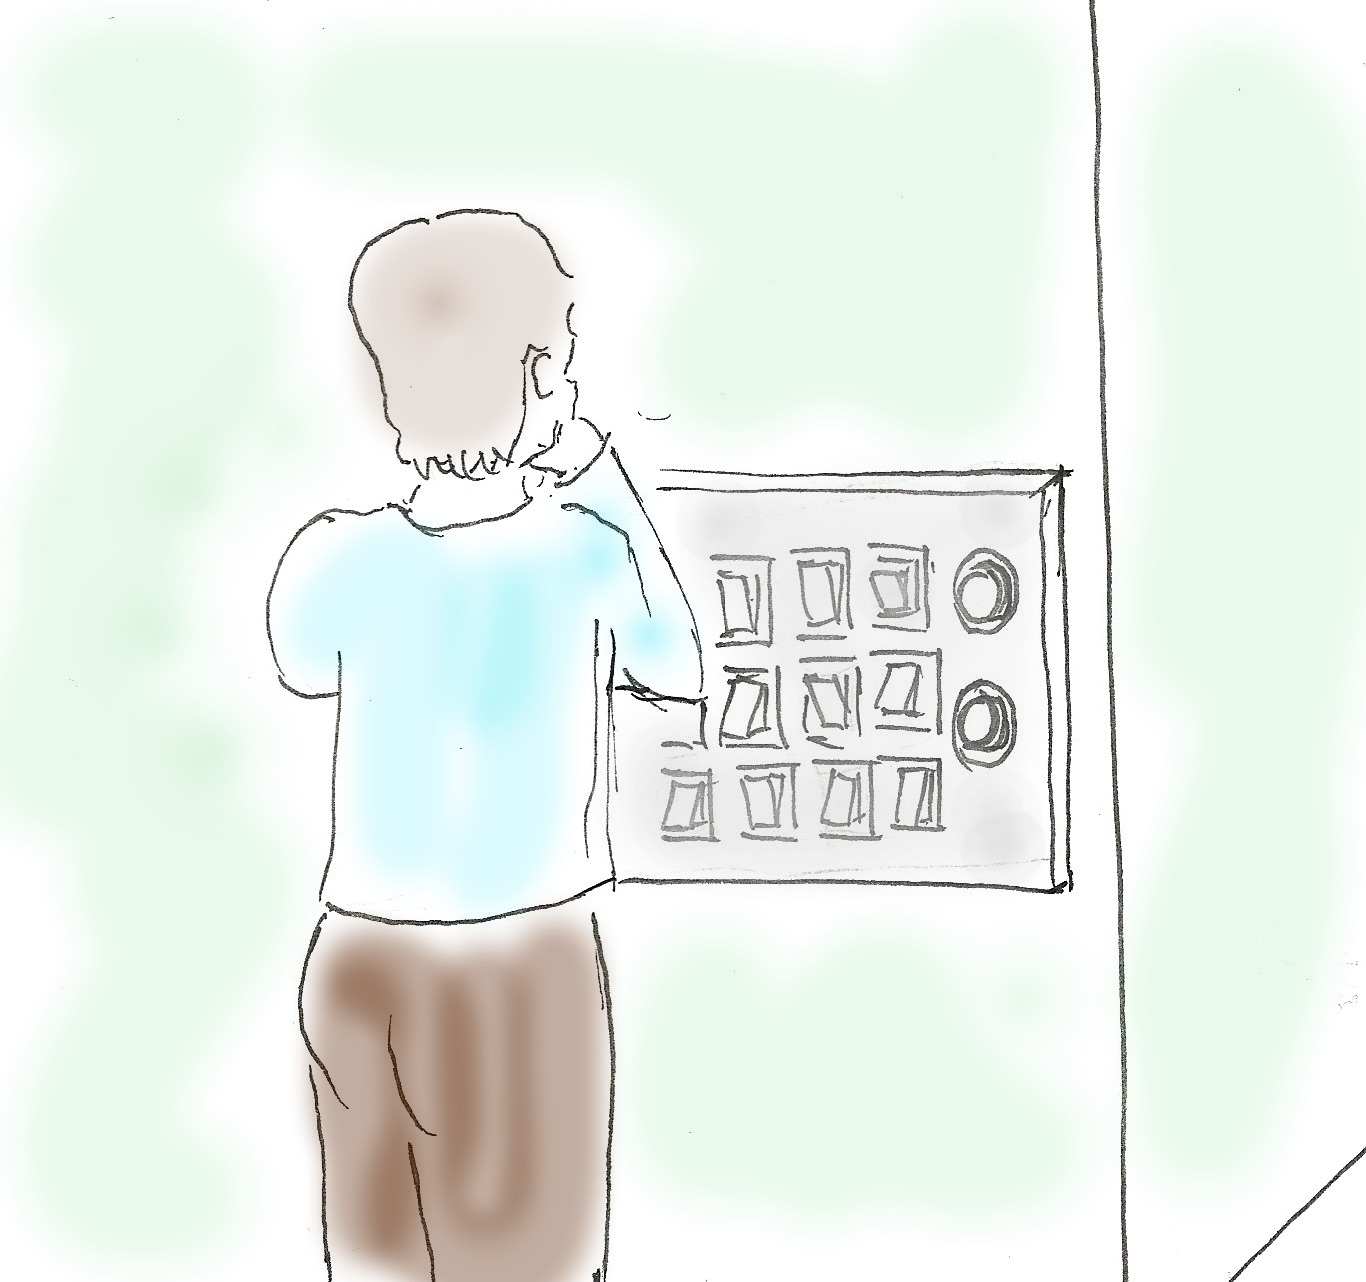
\includegraphics[scale=0.2]{fig/confusingbuttons}
\caption{Stort panel med knapper skaper forvirring.}
\label{fig:panel}
\end{figure}\\
\textbf{Hypotese 1 - Gestegjenkjennelse gjennom fotodioder}\\
\emph{En enkel sensor med fotodioder kan benyttes som en multifunksjonell, mekanisk bryter, og bruk av maskinlæring kan gi sensoren evnen til å skille mellom flere kommandoer enn eksplisitt programmering kan.}\\\\
Programvare for å forstå tale blir stadig bedre. Desverre er det et stort problem å lage et brukbart system i scenarier der programvaren skal lytte etter kontinuerlig tale og må kunne skille mellom hva som er en kommando, og hva som kun er ordinær tale mellom mennesker. Det ville for eksempel vært et problem dersom alle som kom hjem på besøk måtte få en innføring i alle ord som ville utløse kommandoer og som de ikke kunne bruke mens de var i huset. Kommersielle systemer for talegjenkjenning løser gjerne dette ved å lytte etter et kodeord, men med denne tilnærmingen forsvinner drømmen om å ha en kontinuerlig dialog med datamaskinen. Forståelse av naturlig språk har et annet stort problem; prosesseringen og forståelsen av taledata må foregå i kraftige serverparker langt unna brukeren. Dette er et problem med tanke på personvern og det er et praktisk problem med en ikke ubetydelig ventepause før resultatet returneres til brukeren. Kanskje det ikke er nødvendig å forstå naturlig, kontinuerlig tale for å tilby kontroll over hjemmet?\\\\
\textbf{Hypotese 2 - Multimodal interaksjon gjennom tale og gester}\\
\emph{Kombinasjonen av enkle gester og begrenset tale er en tilstrekkelig, naturlig og effektiv måte å kontrollere hjemmet på.}\\\\
En gest utført foran flere sensorer i en viss konfigurasjon vil skape mer data. Det virker derfor rimelig å anta at mer data kan lede til en enda mer nøyaktig forståelse av ulike kommandoer. Sensorene har også muligheten til å måle andre verdier, som lys-nivåer, nærhet og tilstedeværelse. Kan disse egenskapene utnyttes i et smart hjem?\\\\
\textbf{Hypotese 3 - Kombinasjoner}\\
\emph{Ved å benytte flere sensorer i kombinasjon kan man oppnå en høyere presisjon enn ved bruk av en enkelt sensor, flere kommandoer kan utføres naturlig og sensorenes evne til å måle lys, nærhet og tilstedeværelse kan også utnyttes verdifullt i et smart hjem.}\\\\
Standard programvare for styring av smarte hjem er i dag grafiske brukergrensesnitt der metaforiske objekter, som knapper og brytere skal manipuleres. Er dette egentlig nødvendig? Brukerne bryr seg ikke om disse kunstige objektene. De bryr seg om informasjonen om hjemmet og om å forstå valgene de kan ta. Den eneste modellen som skal manipuleres befinner seg i hodene deres. Et grafisk brukergrensesnitt for smarte hjem er informasjonsprogramvare og bør designes som en informasjonsgrafikk og ikke som manipulasjonsprogramvare.\\\\
\textbf{Hypotese 4 - Kontekstdrevet brukergrensesnitt}\\
\emph{Et grafisk brukergrensesnitt for det smarte hjemmet bør være kontekstsensitivt og være drevet av data, ikke interaksjon med brukeren.}

\subsection{Design av eksperimenter}

\subsubsection*{Gestegjenkjennelse gjennom fotodioder}
For å teste denne hypotesen må det først finnes fram en aktuell sensor og deretter etablere at den kan benyttes som en multifunksjonell mekanisk bryter. Med dette grunnlaget kan man utforske dataene sensoren produserer. Deretter kan dataene prosesseres og programvare kan utvikles for å lære forskjellene i dataene ulike gester produserer. Resultatene fra et slikt system må være tilsvarende eller bedre enn resultatene fra et eksplisitt programmert system. Det er to dimensjoner til dette resultatet: antallet ulike gester systemet kan skille mellom og hvor ofte gestene forstås korrekt.

For å gjennomføre eksperimentet trengs det tilgang til en sensor som produserer tilstrekkelig detaljert data når et objekt føres i nærheten. Dataene må overføres fra sensoren til en kraftigere datamaskin. Her må dataene behandles og forberedes til maskinlæring. Til slutt trengs det gode biblioteker for læringen, gjerne med en rekke tilgjengelige algoritmer så flere tilnærminger kan forsøkes. Maskinlæringsalgoritmer er sjeldent svært avanserte og vanskelige å implementere, men for å oppnå gode resultater hurtig trengs optimaliserte implementasjoner. Det virker derfor rimelig å lete etter passende biblioteker, framfor å implementere egne algoritmer.

\subsubsection*{Multimodal interaksjon gjennom tale og gester}
I mangelen på tilgang til empirisk brukertesting kan denne hypotesen utfordres med argumentasjon. Først må det etableres at dagens løsninger for kontinuerlige tale har problemer med personvern og responstid. Videre må det argumenteres for at enkle gester og begrenset tale fungerer godt til å styre hjemmet. Til slutt må det vises hvordan eventuell multimodal input kan håndteres og gi tilfredsstillende resultater.

Dersom eksperiment 1 er en suksess er gestegjenkjennelse tilgjengelig. Videre må det velges eller implementeres et system for talegjenkjenning. Det trengs i tillegg til utstyret fra eksperiment 1 en mikrofon for å lytte etter tale. Det trengs også teknikker for å håndtere data fra gester og tale samtidig. Å håndtere simultan data fra både gester og tale er et problem. Hvordan sikrer man at data ikke går tapt dersom input kommer samtidig fra begge kilder? Hvilken data skal ha prioritet dersom de kommer samtidig? Til sist bør eksperimentet visualiseres på et vis for å vise at systemet fungerer slik som ønsket.

\subsubsection*{Kombinasjoner}
Maskinlæring må benyttes igjen i dette eksperimentet og bruken av flere sensorer må gi et betydelig bedre resultat i en eller begge av dimensjonene jeg har nevnt. Deretter må det kunne vises at de andre egenskapene ulike enkle sensorer har kan benyttes produktivt i forbindelse med et smart hjem. Dette kan kun argumenteres.

Jeg tar utgangspunkt i at eksperiment 1 og 2 har vært vellykkede. Det trengs flere sensorer, og eventuelt annen hardware for å håndtere disse. Posisjonen til sensorene er interessant. Skal de plasseres så nære hverandre som mulig, for å fungere som en enkelt bryter med større presisjon? Eller skal de posisjoneres et godt stykke fra hverandre, så de kan benyttes med begge hender og som en enkelt eller delvis flere brytere?

\subsubsection*{Kontekstdrevet brukergrensesnitt}
Denne siste hypotesen testes ved å implementere et grafisk brukergrensesnitt og vise hvordan det i dette scenariet er overlegent tradisjonelle, interaksjonsdrevne systemer. Hypotesen omhandler informasjonsprogramvare; hvordan relevant informasjon om hjemmet kan presenteres for brukeren. For å implementere eksperimentet må det velges teknologi for å lage et brukergrensesnitt. Aktuelle muligheter er webteknologi, animasjon av et slag, eller programvare til desktop eller app-er. Det trengs teknologi med evnen til å forandre seg basert på data og ikke nødvendigvis interaksjon med brukeren. \\

\subsection{Implementasjon}

\subsubsection{Gestegjenkjennelse gjennom fotodioder}
For å implementere eksperimentet har jeg brukt sensoren \emph{APDS-9960} fra Avago Technologies\footnote{\url{http://www.farnell.com/datasheets/1801560.pdf}}. Denne sensoren har flere funksjoner og tilbyr måling av lys og farge, oppdagelse av nærhet og gestegjenkjennelse. Innpakningen er svært liten på kun 3.94 * 2.36 * 1.35 mm, og kan ses i figur \ref{fig:sensor-size}. Gestesensoren selv består av fire fotodioder, som kan oppfatte et infrarødt signal. En LED sender ut det infrarøde signalet og dersom et objekt befinner seg innenfor omtrent 20 cm vil signalet reflekteres tilbake med nok styrke til å bli oppfattet av fotodiodene. Fotodiodene er vinklet litt forskjellig slik at de plukker opp refleksjoner fra ulike retninger. Gestesensoren benytter resultater fra en nærhetsdetektor for å automatisk aktiveres når et objekt er innen rekkevidde. I tilegg brukes måling av lys for å tilpasse de infrarøde målingene til lysnivået i omgivelsene. Disse egenskapene gjør denne sensoren mer nøyaktig enn enklere varianter som benytter én LED og én fotodiode (som keyboardet beskrevet av \citet{96bytes}). Dataene dannes som 32-bit datasett og kommuniseres over I2C-protokollen til en mikrokontroller. For å utvikle systemet er \emph{Sparkfun}'s innpakning av APDS-9960-sensoren benyttet\footnote{\url{https://www.sparkfun.com/products/12787}}. Figur \ref{fig:sensor-size} viser APDS-9960-sensoren på Sparkfun-brettet. Dette brettet gjør sensoren tilgjengelig for enklere prototyping ved å bryte ut ulike pinner. I tillegg har Sparkfun skrevet programvare til \emph{Arduino}-plattformen\footnote{\url{http://www.arduino.cc/}} så utviklere kommer raskt i gang og kan gjøre bruk av de forskjellige funksjonalitetene hos APDS-9960-brikken.
\begin{figure}[h]
\centering
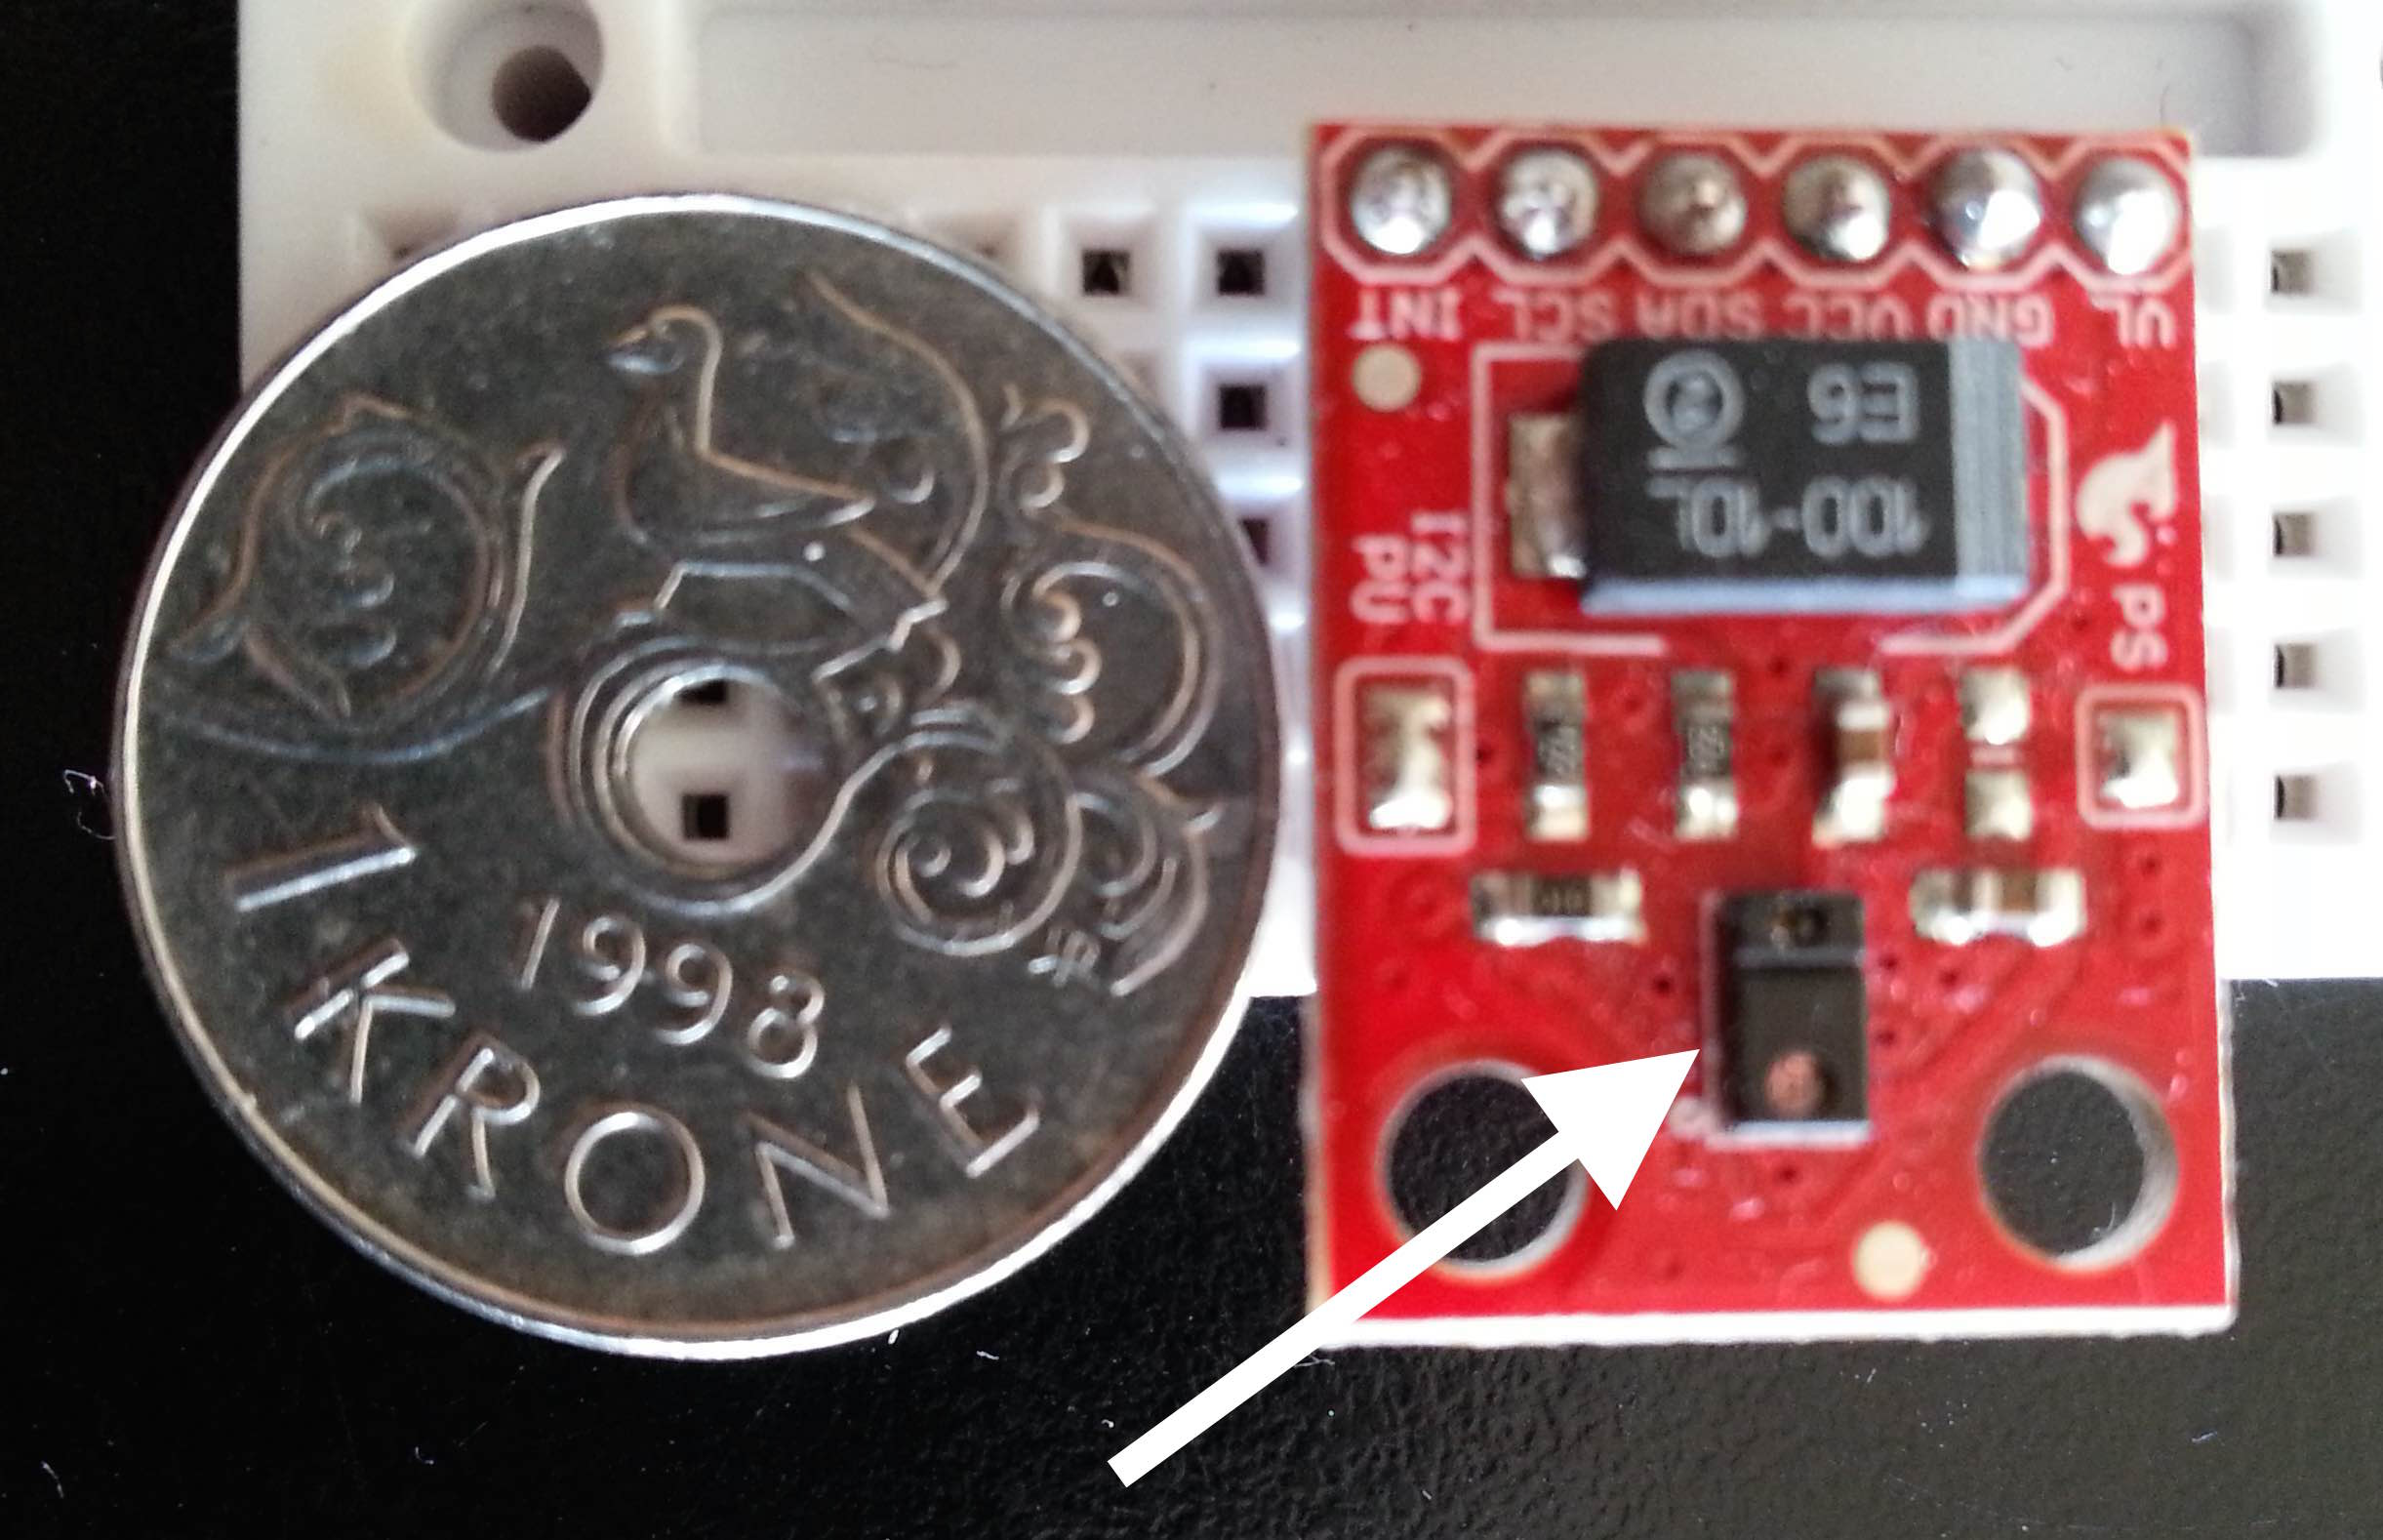
\includegraphics[width=7.5cm, height=5cm]{fig/sensor-size}
\caption{Sensorstørrelse: APDS-9960, montert på Sparkfun-brettet.}
\label{fig:sensor-size}
\end{figure}

\begin{table}[h!]
\caption{Utstyrsliste eksperiment 1}
\centering
\begin{tabular}{|| c c ||}
\hline
 Utstyr & Bruksområde \\
 \hline\hline
 Sparkfun APDS-9960 & Gestesensor \\ 
 \hline
 Level-shifter & Konverterer mellom 5V og 3.3V \\
 \hline
 Breadboard & Montere sensor og level-shifter for enklere prototyping \\ 
 \hline
 Break-away headers & Montere sensor og level-shifter til breadboard   \\ 
 \hline
 Loddebolt og tinn & Lodde headers til sensor og level-shifter\\
 \hline
 Ledninger & Overføre signal mellom sensor, level-shifter og Arduino \\
 \hline
 Arduino Uno & Drive sensoren og sende data til datamaskinen\\
 \hline
 USB-kabel & Overføre data til datamaskinen \\
 \hline
 Macbook Pro & Håndtere data og utføre maskinlæring\\
 \hline
\end{tabular}
\label{table:utstyrsliste}
\end{table}
For å trene systemet kreves data og for å få dataene inn til datamaskin kreves en mikrokontroller. Med Sparkfuns programvare for Arduino var det naturlig å velge en Arduino som mikrokontroller. Arduinoen ble koblet til sensoren ved å følge oppkoblingsguiden på hjemmesidene til Sparkfun\footnote{\url{https://learn.sparkfun.com/tutorials/}}. Gestesensoren drives på 3.3V, mens en normal Arduino Uno drives på 5V. Dermed ble det nødvendig å introdusere en level-shifter, for å konvertere fra 5V til 3.3V. Tabell \ref{table:utstyrsliste} viser eksperimentets utstyrsliste. Figur \ref{fig:single-sensor} viser hvordan komponentene ser ut etter å ha blitt koblet sammen og er klargjort for å utføre eksperimentet.

Etter at Arduinoen, sensoren og datamaskinen har fått kontakt kan jeg benytte programvaren til Arduino-plattformen til å laste opp koden som trengs for å drive sensoren. Jeg tilpasset biblioteket fra SparkFun minimalt, slik at Arduinoen ikke selv forsøker å forstå sensordataene, men i stedet sender dataene videre til datamaskinen.
\begin{figure}[h]
\centering
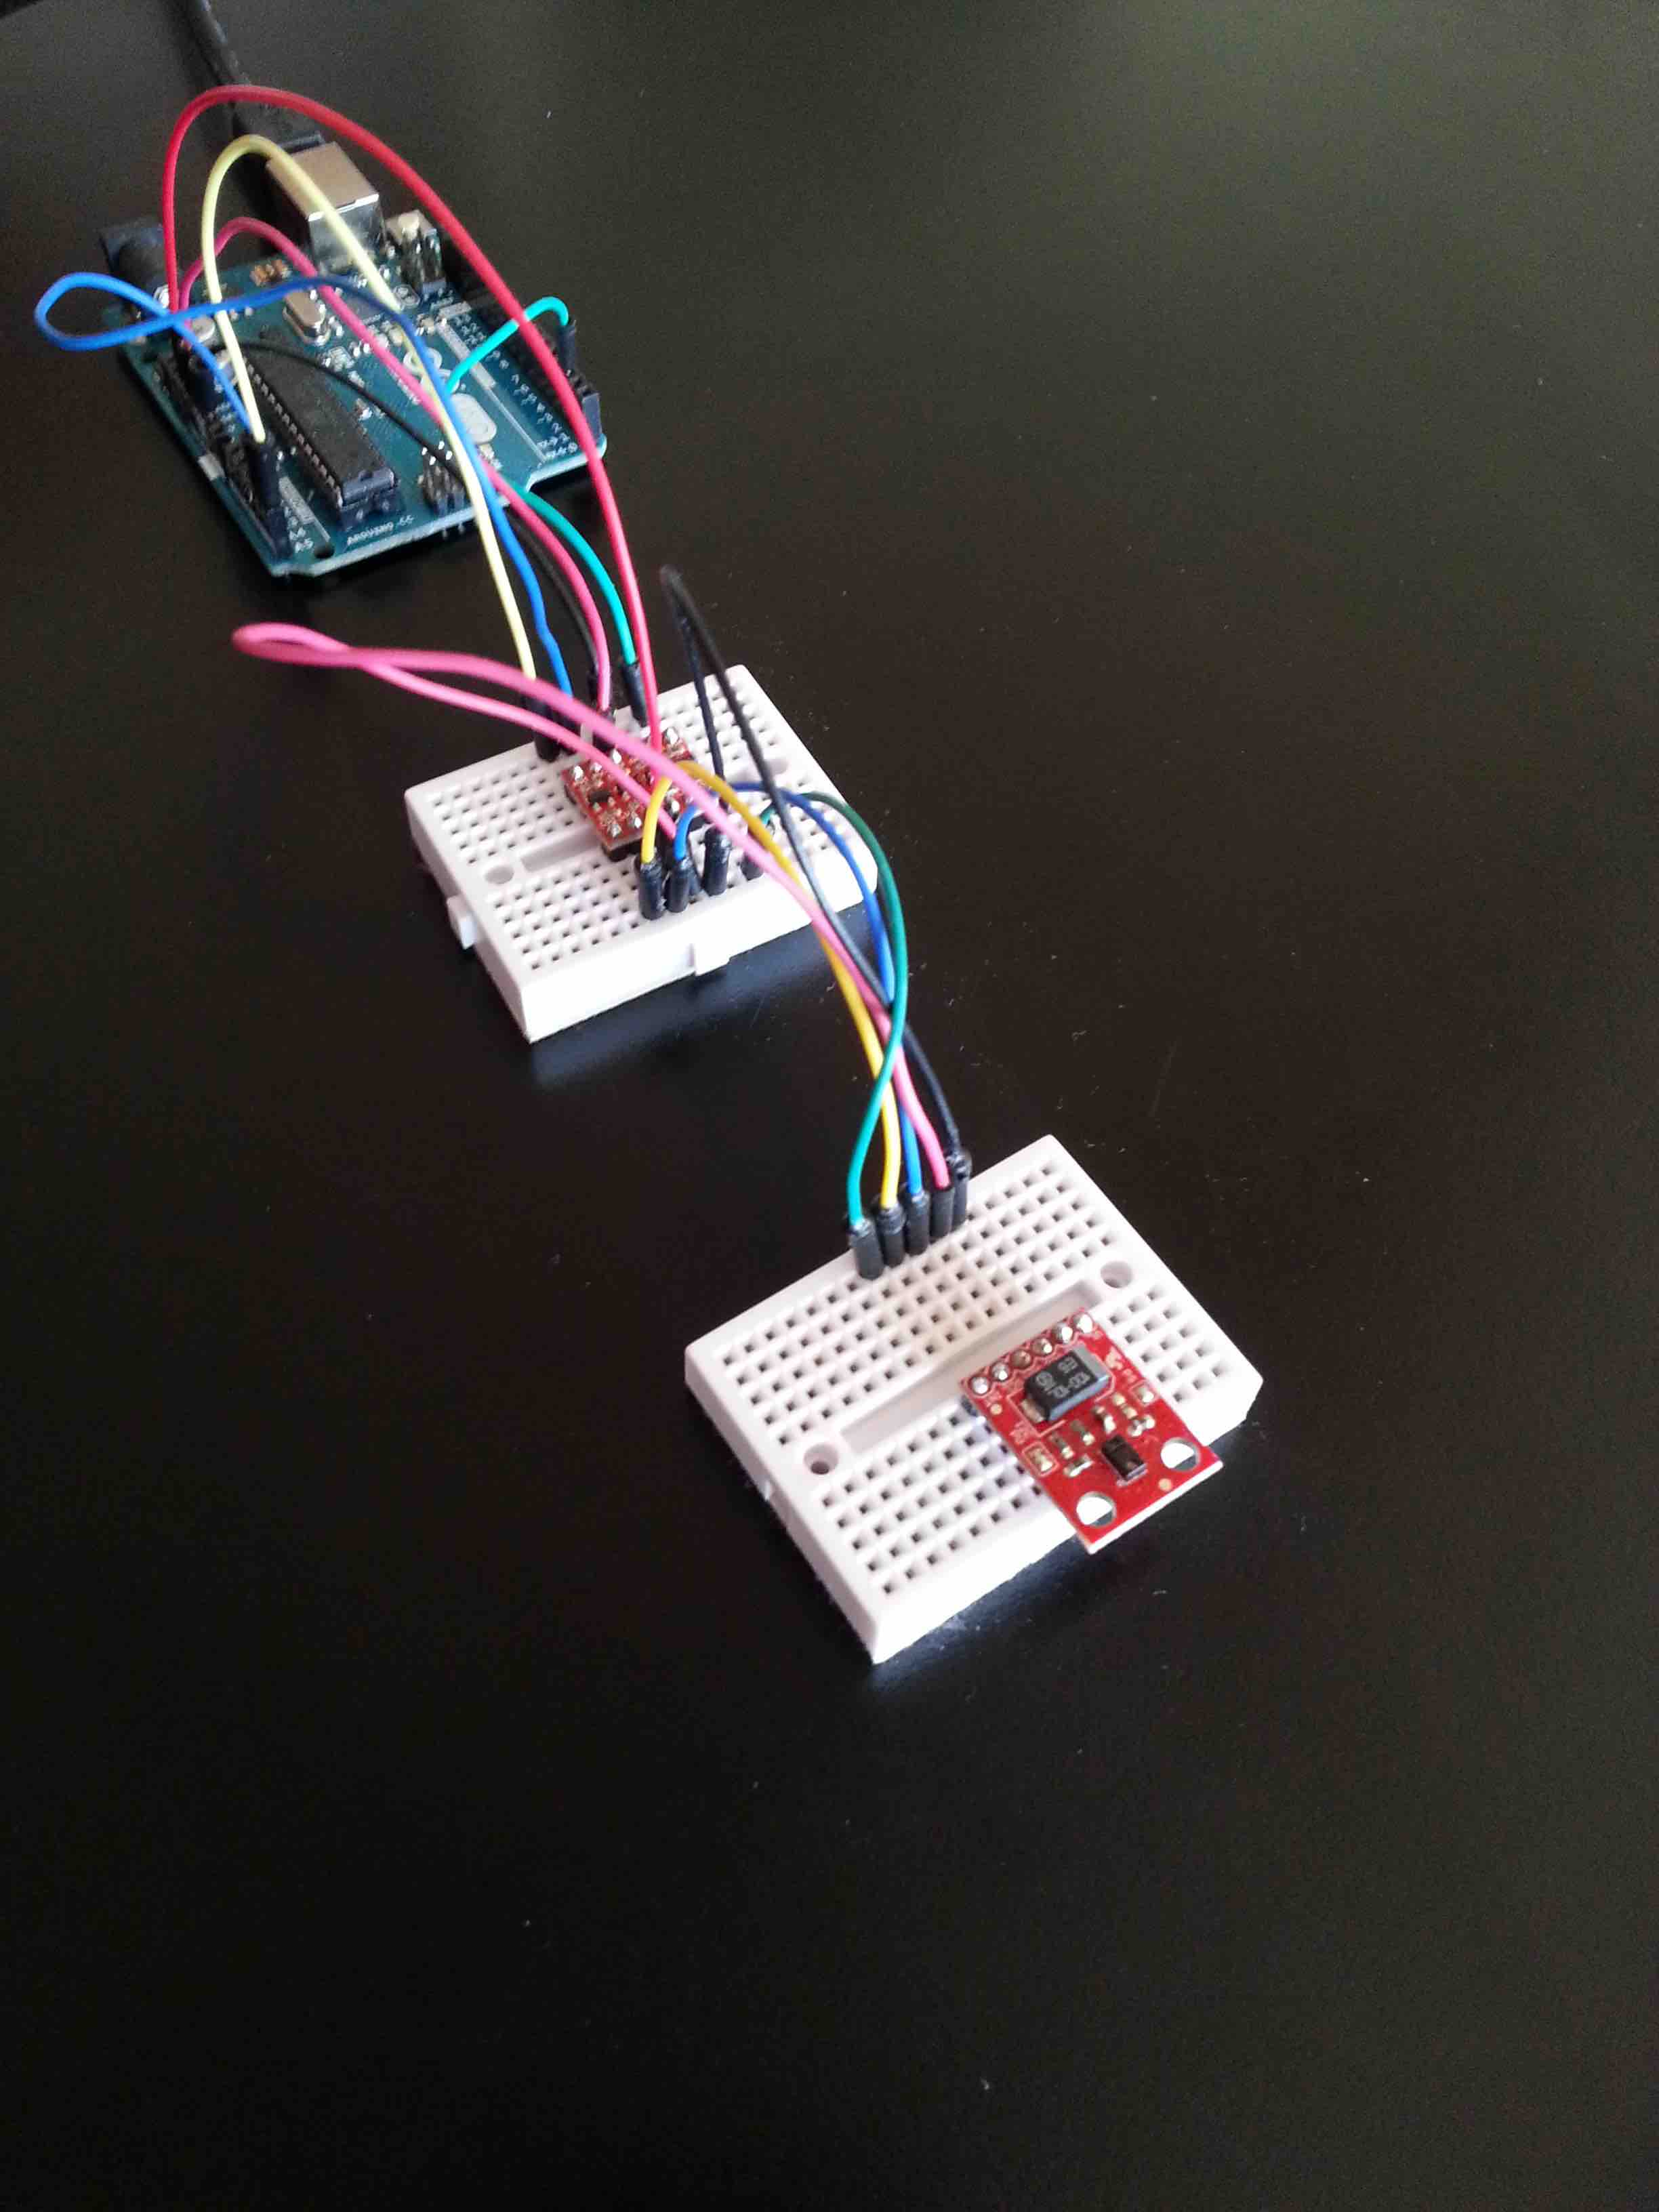
\includegraphics[width=10cm, height=10cm]{fig/singlesensor}
\caption{Sensor, level shifter og Arduino.}
\label{fig:single-sensor}
\end{figure}
For å håndtere dataprosesseringen og utføre maskinlæring valgte jeg programmeringsspråket \emph{Python}\footnote{\url{http://www.python.org}}. Dette valget ble tatt med utgangspunkt i at Python har et bredt utvalg biblioteker innen både seriell kommunikasjon og maskinlæring. Jeg vurderte noen alternativer og gjorde noen utforskende forsøk med å benytte Java-plattformen og et av språkene som kjører på JVM. Java har mange gode biblioteker, spesielt innen maskinlæring. Desverre støtte jeg på problemer med å håndtere den serielle kommunikasjonen. Jeg antar at bruken av en virtuell maskin skaper noe mer kompleksitet rundt å kommunisere via de noe utdaterte serielle portene. Et siste alternativ jeg vurderte var å benytte programmeringspråkene Matlab eller R, som begge er populære verktøy innen AI. Igjen viste det seg at Python hadde et fortrinn når det gjaldt den serielle kommunikasjonen.

Arduino-programvaren henter data via I2C-protokollen fra sensoren. Den sender så dataene videre serielt til datamaskinen som lytter på den aktuelle porten. Sensoren sender data så lenge det infrarøde signalet reflekteres og oppfattes av fotodiodene. Dette betyr at en gest som tar lengre tid skaper mer data. Et raskt flikk med to fingre skaper 16-32 datapunkter. Et rolig sveip over sensoren med hele hånda kan skape 100-200 datapunkter. En gest som involverer å holde hånda foran sensoren i flere sekunder skaper hundrevis av datapunkter. Den variable mengden datapunkter skaper et problem; for å benytte de planlagte klassifiseringsteknikkene må hvert av treningseksemplene må ha like mange datapunkter.

Det finnes ulike metoder for å løse dette problemet. En løsning er å bestemme det maksimale antallet datapunkter som skal tas med. Inputeksempler som ikke har tilstrekkelig med datapunkter får lagt til 0-verdier for å oppnå den ønskede størrelsen. Å sette en slik maksgrense på datapunkter kan desverre føre til at man mister viktig data fra gester som tar lengre tid å utføre. Og for et inputeksempel fra en rask gest vil mange datapunkter være 0. Disse problemene kan påvirke effektiviteten til læringsalgoritmen. Et annet alternativ er å velge et fast antall datapunkter vært inputeksempel skal ha. Deretter knytter man inputeksempelet til denne vektoren av fast størrelse. Dersom inputdataene har få datapunkter blir den resulterende vektoren sparsom, med dataverdiene spredt jevnt utover, og med 0-verdier i mellom. Dersom inputdataene består av mange datapunkter vil hvert datapunkt i vektoren være et gjennomsnitt av en valgt mengde datapunkter.

Jeg valgte å benytte denne sistnevnte teknikken og lagde vektorer med 128 datapunkter. Dette tallet ble valgt basert på tester av ulike aktuelle gester og antallet datapunkter disse genererte. 128 datapunkter er nok til å gi tilstrekkelig detaljer selv ved gester som tar noe lengre tid og samtidig ikke så mange at raske gester skaper i overkant sparsomme vektorer. Vektoren normaliseres ved å knytte de mulige sensorverdiene [0,255] til [0.0,1.0]. Å illustrere dannelsen av vektorer med 128 datapunkter blir tungvint så i figur \ref{fig:data} har jeg illustrert prosessen med langt mindre data. I \ref{fig:few} består inputvektoren av to datapunkter. La oss si vi ønsker en vektor med størrelse fire og som er normalisert til verdiområdet [0.0,10.0]. Dette oppnås ved å spre inputdataene jevnt i vektoren og normalisere verdiene. \ref{fig:many} viser det motsatte tilfellet, der inputvektoren er for stor. For å representere dataene i en mindre vektor blir det tatt gjennomsnittsverdier som deretter normaliseres.
\begin{figure}[h]
\centering
\begin{subfigure}{0.44\textwidth}
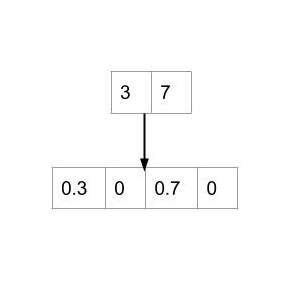
\includegraphics[width=6cm, height=6cm]{fig/process1}
\caption{}
\label{fig:few}
\end{subfigure}
\begin{subfigure}{0.44\textwidth}
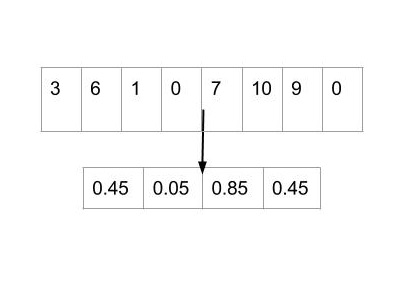
\includegraphics[width=8cm, height=6cm]{fig/process2}
\caption{}
\label{fig:many}
\end{subfigure}
\caption{Dannelsen av en datavektorer.}
\label{fig:data}
\end{figure}
\begin{listing}[ht]
\caption{Dataprosessering}
\inputminted[fontsize=\footnotesize, linenos]{python}{kodesnutter/preprocess_data.py}
\label{code:dataprocessing}
\end{listing}
Listing \ref{code:dataprocessing} viser koden som prosesserer dataene og forbereder dem på maskinlæringen. På linje 3 dannes det en vektor med 128 0-verdier. Linje 4 avgjør om inputdataene skal spres jevnt i resultatsvektoren eller om det skal dannes gjennomsnittsverdier.

Eksperimentet vil ha to deler. Den første delen blir å utføre en rekke eksempler på gester og lagre de prosesserte dataene. Del to er å laste inn dataene og danne en modell som kan trenes, testes og evalueres. For å utføre maskinlæringen benyttet jeg to Python-biblioteker: \emph{NumPy}\footnote{\url{http://www.numpy.org/}} og \emph{scikit-learn}\footnote{\url{http://scikit-learn.org/stable/}}. Numpy er det mest brukte biblioteket for numeriske kalkulasjoner i Python. For maskinlæringen finnes det mange alternativer. Scikit-learn ble valgt fordi det tilbyr et stort utvalg algoritmer og er spesielt gode på de lineære klassifiseringsalgoritmene. For å benytte klassifiseringsalgoritmene scikit-learn har tilgjengelig trengs det to NumPy-datasett: et datasett med dataene fra gestene, og et tilsvarende med tilhørende klasser.
\begin{listing}[ht]
\caption{Splitte datasettene}
\inputminted[fontsize=\footnotesize]{python}{kodesnutter/split_data.py}
\label{code:split}
\end{listing}
Listing \ref{code:split} benytter \emph{kryssvalidering} til å splitte dataene (X) og klassene (y) inn i trenings- og testsett. Jeg valgte å dele datasettene i 75\% til trening og 25\% til testing.\\

\subsubsection{Multimodal interaksjon gjennom tale og gester}
\label{ch:multimodalimpl}
Det finnes alternativer dersom man ønsker å utforske programvare for talegjenkjenning. Blant andre tilbyr \emph{Google} sitt tale-API til interessenter. Min idé er at disse tjenestene muligens ikke er det vi ønsker i hjemmet, så vi må ty til andre midler. Dette eksperimentet handler delvis om å argumentere hvorfor dette er tilfellet og blir greid ut om i kapittel 4. 

Hva er statusen på talegjenkjenningsteknologi som ikke benytter internettkommunikasjon med kraftige servere? Etter en utforskning av alternativene valgte jeg å benytte Pocketsphinx, en av talegjenkjenningsmotorene fra Carnegie Mellon University's Sphinx-prosjekt\footnote{\url{http://cmusphinx.sourceforge.net/}}. \emph{CMU Sphinx} er et pågående, åpent prosjekt og de har to aktuelle prosjekter for talegjenkjenning: \emph{Sphinx4} og \emph{Pocketsphinx}. Pocketsphinx er designet for mobile enheter og andre alternative, ressursbegrensede plattformer. Den har et konfigurerbart vokabular så man kan skape modellene man trenger. I følge en nylig skrevet artikkel kan Pocketsphinx med god konfigurering gjenkjenne 10000 ord i reelltid med en feilrate på omtrent 20\%\footnote{\url{http://cmusphinx.sourceforge.net/2015/02/}}. Dette er teknisk imponerende for denne ressurseffektive programvaren, men det er en for stor feilrate til å være praktisk i kommersiell bruk. Heldigvis øker presisjonen betydelig med et mindre vokabular og med under 100 ord er feilraten 3\%. Pocketsphinx tilbyr også å benytte et aktiveringsord, slik at enheten kan lytte kontinuerlig gjennom dagen.

Sphinx4 er skrevet i Java og ble utforsket i forbindelse med å utføre både gesteforståelse og talegjenkjenning på Java-plattformen. Pocketsphinx er skrevet i \emph{C} og er dermed lettere tilgjengelig for bruk gjennom Python. Etter at jeg hadde avgjort å jobbe med Python ble Pocketsphinx det naturlige valget. For å benytte Pocketsphinx trengs det tre datakilder: en HMM, en språkmodell og en ordbok. CMU Sphinx-prosjektet utvikler stadig nye HMM-modeller og den engelske er godt moden. Desverre har de ikke jobbet med en norsk modell. Det finnes modeller for norsk der ute, men da jeg ikke fant noen åpne og fritt tilgjengelige ble jeg tvunget til å utføre eksperimentet på engelsk. Dette var ikke et problem, da eksperimentet handler om argumentasjon for lokal og begrenset talegjenkjenning og den praktiske utførelsen av multimodalitet, ikke språket det tales i. Språkmodellen og ordboken er basert på en liste over ord eller setninger som talegjenkjenningen skal forsøke å forstå lyder som. CMU Sphinx tilbyr et verktøy\footnote{\url{http://www.speech.cs.cmu.edu/tools/}} for å lage en språkmodell og ordbok, basert på en liste over aktuelle setninger. Modellen som dannes kan forstå kombinasjoner av ordene og setningene, men kombinasjonen man faktisk skriver inn i lista blir vektet tyngre.

For å håndtere simultan input fra begge datakilder valgte jeg å benytte tråder og en felles FIFO-kø. Hovedtråden i programmet starter to nye tråder som hver har ansvar for å drive input-funksjonene til gestedata og taledata. 
\begin{listing}[ht]
\caption{Bakgrunnstråder}
\inputminted[fontsize=\footnotesize, linenos]{python}{kodesnutter/background_threads.py}
\label{code:backgroundthreads}
\end{listing}
Listing \ref{code:backgroundthreads} definerer en funksjon som tar en funksjon og argumenter som input, og starter en bakgrunnstråd som utfører funksjonen med argumentene.
\begin{listing}[ht]
\inputminted[fontsize=\footnotesize, linenos]{python}{kodesnutter/gesture_data.py}
\caption{Overføre data fra gester}
\label{code:gesturedata}
\end{listing}
Funksjonene i bakgrunnstrådene henter data fra seriellporten for gestedata, og fra mikrofonen for taledata. Disse dataene puttes på en felles kø, som en \emph{tuple}: et kodeord, sammen med dataene. På denne måten blir dataene merket slik at forbrukeren av køen kan skille mellom kildene dataene kommer fra. Hovedtråden lytter etter ny data på køen. På denne måten er de to inputkildene likestilte. Listing \ref{code:gesturedata} viser funksjonen som håndterer input fra gestesensoren. \emph{While}-løkken bygger opp en databuffer. Når alle dataene som representerer en gest har ankommet fra sensoren puttes de på køen sammen med en etikett som forteller om datakilden.

Hovedtråden driver en animasjon. Animasjonen utføres av \emph{pyprocessing}\footnote{https://code.google.com/p/pyprocessing/}, et bibliotek som følger animasjonsspråket \emph{Processing}'s konvensjoner.
\begin{listing}[ht]
\caption{Håndtere multimodal inputdata}
\inputminted[fontsize=\footnotesize, linenos]{python}{kodesnutter/multimodal.py}
\label{code:multimodal}
\end{listing}
Det første elementet i data-tuplen er et kodeord. Dersom kodeordet sier at dataene er gestedata tegnes det på et vis, og dersom dataene er taledata på et annet. Dersom det ikke er ny data i køen tegnes ingenting nytt.

Denne implementasjonen viser hvordan to inputkilder enkelt kan operere asynkront og dytte data inn på en felles kø. Hovedtråden i programmet henter data fra køen og avhengig av kilden tegnes dataene forskjellig på skjermen. Implementasjonen viser et enkelt alternativ til hvordan multimodal input kan håndteres.\\

\subsubsection{Kombinasjoner}
\begin{figure}[h]
\centering
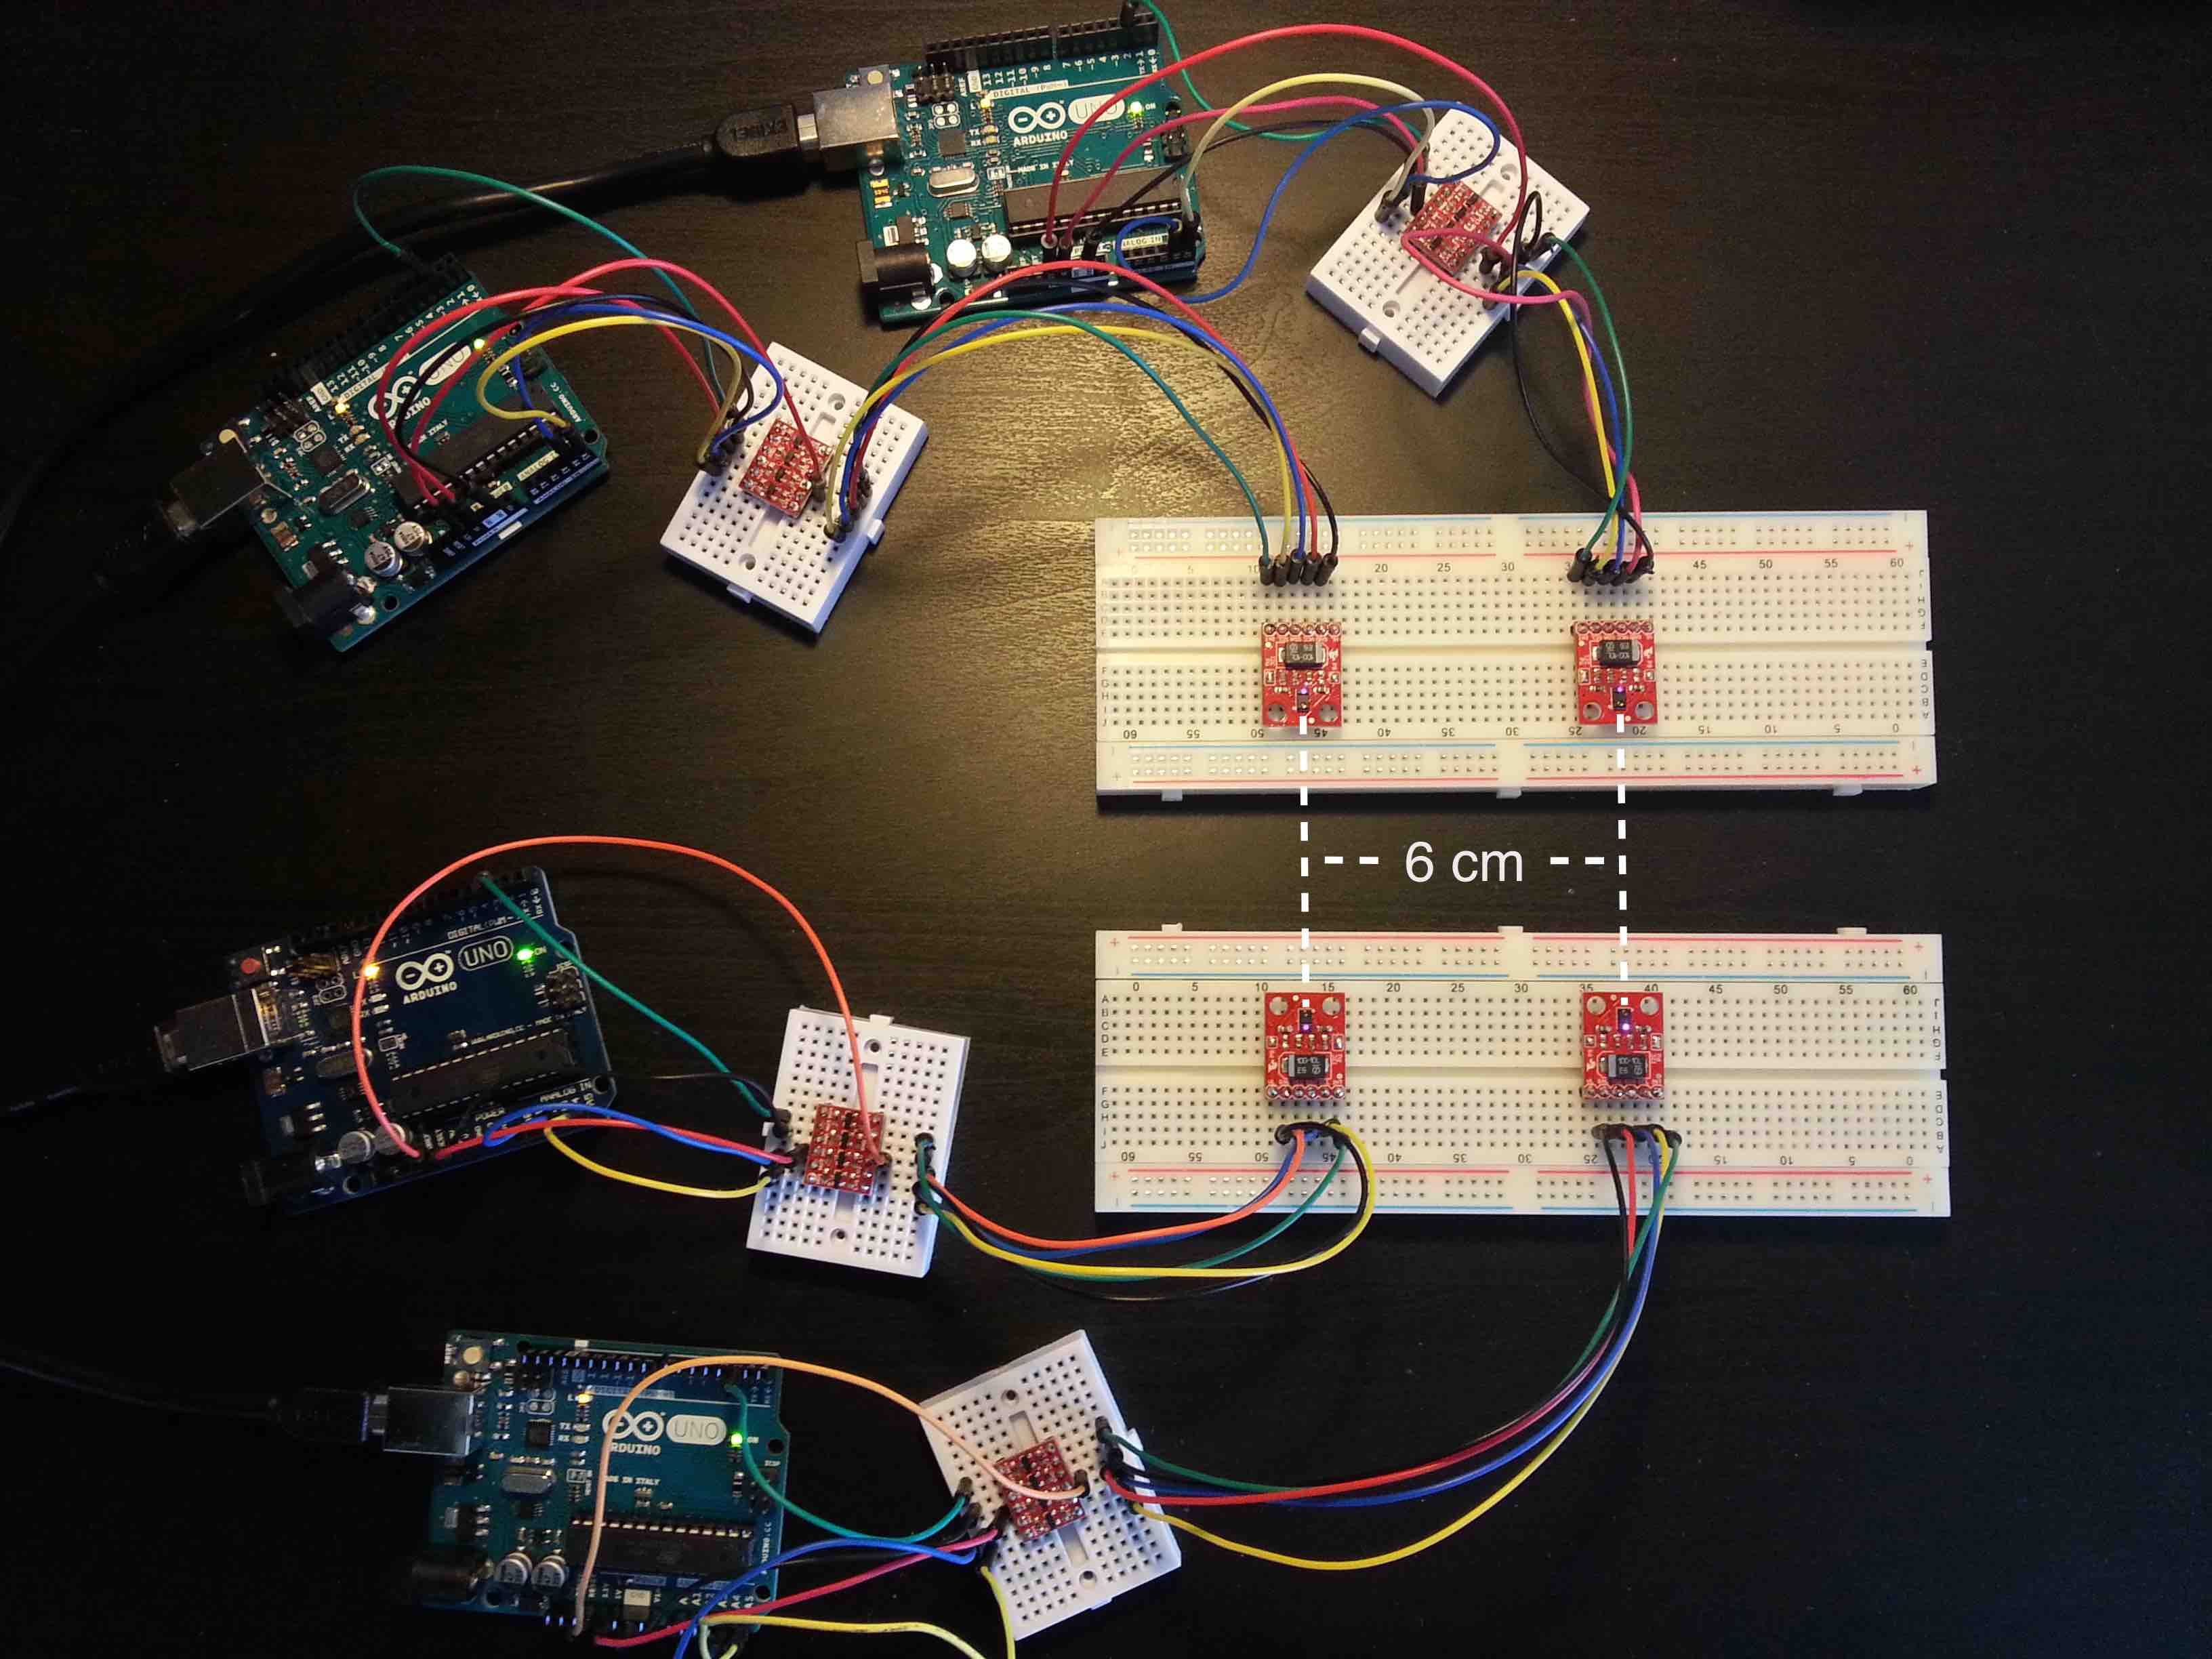
\includegraphics[width=15cm, height=12cm]{fig/foursensors}
\caption{Fire sensorer.}
\label{fig:four-sensors}
\end{figure}
Jeg valgte å benytte fire sensorer, der selve sensorene danner hjørner i et kvadrat på 6 * 6 cm, som vist i figur \ref{fig:four-sensors}.
For å håndtere data fra fire sensorer samtidig valgte jeg å benytte samme strategi som i eksperiment 2; fra hovedtråden i programmet starter jeg opp fire tråder som hver lytter på sin port, og dytter data fra gestesensorene inn på en felles kø. Hovedtråden henter data fra køen helt til køen er tom.

De individuelle trådene putter også her dataene på køen sammen med en identifikator, så hovedtråden forstår hvor dataene har sitt opphav. Ettersom dataene fra de ulike sensorene kan komme i en uforutsigbar rekkefølge er jeg nødt til å sortere. Hovedtråden bygger opp lister av data fra hver sensor. Når køen er tom prosesseres rådataene og forberedes til maskinlæringen. Jeg valgte også her å benytte vektorer med størrelse på 128 datapunkter, for hver sensor. \begin{listing}[ht]
\caption{Dimme lys}
\inputminted[fontsize=\footnotesize, linenos]{python}{kodesnutter/dimming.py}
\label{code:dim}
\end{listing}Dette betyr at dersom en gest for eksempel kun blir oppfattet av en av de fire sensorene, vil den resulterende vektoren på 512 datapunkter ha minimum 364 datapunkter som er null. På denne måten vil systemet svært enkelt lære gester som kun aktiverer et subsett av de fire sensorene. Maskinlæringen er tilsvarende i eksperiment 1; scikit-learn håndterer inputdata med vilkårlig store datavektorer.

Listing \ref{code:dim} viser hvordan eksperimentet med nærhetssensoren og dimming kan håndteres. Data fra nærhetssensoren kommer inn til hovedtråden kontinuerlig, men det er først når det riktige ordet ytres og talegjenkjenningen gjenkjenner dette at nærhetsdataene blir brukt. Ved å si "lights" og holde hånda foran sensoren kan brukeren dimme lysnivået.

\subsubsection{Kontekstdrevet brukergrensesnitt}
Det var klart at teknologi med av en dynamisk natur burde benyttes i implementasjonen av dette eksperimentet. Det mest dynamiske ville vært animasjonsteknologi, men ettersom brukergrensesnittet bare trenger å oppdatere dersom det er ny data, virket webteknologi som et bedre valg. Jeg valgte å benytte webteknologi \emph{(HTML, CSS, Javascript)}, framfor desktop/app av to grunner: \emph{Javascript}'s dynamiske natur, samt den nokså nye teknologien fra \emph{Facebook} kalt \emph{React}\footnote{\url{https://facebook.github.io/react/}}. React tilbyr et virtuelt \emph{DOM} som man programmerer mot. Når data oppdaterer seg beregner React forskjellen mellom dette virtuelle DOM-et og det virkelige DOM-et. Utregningen av denne forskjellen gjør at minimale deler av det virkelige DOM-et må oppdateres, og det hele er svært effektivt.
\begin{listing}[ht]
\inputminted[fontsize=\footnotesize, linenos]{clj}{kodesnutter/data.clj}
\caption{Datastruktur}
\label{code:datastructure}
\end{listing}
I stedet for å benytte Javascript og React direkte gjorde jeg bruk av \emph{Clojurescript}\footnote{\url{https://github.com/clojure/clojurescript}} og \emph{Reagent}\footnote{\url{https://github.com/reagent-project/reagent}}. Clojurescript er et programmeringsspråk og en \emph{Lisp}-dialekt, som kompilerer til Javascript. Reagent er et Clojurescript-bibliotek for å bruke React. En fordel ved å benytte Clojurescript er at jeg idiomatisk kan modellere hele hjemmets tilstand i en, enkel datastruktur. Først når hjemmets tilstand forandrer seg og denne datastrukturen blir oppdatert, vil React automatisk beregne hvilke deler av det grafiske grensesnittet som må oppdateres.

Listing \ref{code:datastructure} viser deler av datastrukturen. ".." er deler av koden jeg har fjernet for lesbarhet og oversikt. Hjemmets tilstand er representert som et \emph{hash-map}\footnote{En assosiativ datastruktur med konstant tidskompleksitet for lesing og oppdatering}. Nøkkelen \emph{:rooms} har et nytt hash-map som verdi og i dette befinner alle rommene i hjemmet seg. Eksempelrommet \emph{:kitchen} holder data om apparatene og lyset på kjøkkenet. I tillegg til rommene i hjemmet holder datastrukturen annen informasjon om hjemmet, som diagnostikk, vær og brukerpreferanser. Nøkkelen \emph{:view} definerer hvordan det grafiske grensesnittet skal presentere dataene.  
\begin{listing}[ht]
\caption{Atom}
\inputminted[fontsize=\footnotesize, linenos]{clj}{kodesnutter/atom.clj}
\label{code:atom}
\end{listing}
Datastrukturer i Clojurescript er \emph{immutable}; de kan ikke forandres etter dannelse. Listing \ref{code:atom} gjør to ting: den immutable datastrukturen kan nå forandres ved å gå fra en tilstand til en annen, og den er nå koblet til Reacts virtuelle DOM.
\begin{listing}[ht]
\caption{Hovedkonteiner HTML}
\inputminted[fontsize=\footnotesize, linenos]{clj}{kodesnutter/home.clj}
\label{code:home}
\end{listing}
Listing \ref{code:home} er hovedfunksjonen for å generere brukergrensesnittet. Funksjonen returnerer et \emph{div}-element, som puttes inn i HTML-dokumentet brukerens nettleser mottar. På linje 5 spørres det om hvilket \emph{view} som brukes. Dette definerer hvilken HTML-genererende funksjon som skal kalles. For eksempel, dersom \emph{view} er \emph{:kitchen} ser vi at funksjonen \emph{kitchen} kalles med et strengeparameter. Dette vil generere HTML som definerer kjøkkenet og grensesnittet vil zoome inn så detaljene kan ses bedre. Dersom \emph{view} er \emph{:home} kalles alle funksjonene som genererer rom, men med et tomt strengeparameter.

La oss si at \emph{kitchen} ble kalt.\begin{listing}[ht]
\caption{Kjøkken HTML}
\inputminted[fontsize=\footnotesize, linenos]{clj}{kodesnutter/kitchen.clj}
\label{code:kitchen}
\end{listing} Listing \ref{code:kitchen} viser denne funksjonen som også returnerer et \emph{div}-element med videre innhold basert på dataene om hjemmets tilstand. For eksempel bestemmer linje 2 hvilke \emph{CSS}-klasser som skal brukes avhengig av om lyset i hjemmet er av eller på. Denne teknikken brukes for å eventuelt skyggelegge \emph{div}-en som representerer kjøkkenet. Linje 5 definerer kjøleskapet som et bilde. Vi ser at dersom dette bildet trykkes på settes \emph{:food} som verdi til nøkkelen \emph{:view}, i hjemmets tilstand. Denne endringen i hjemmets tilstand vil umiddelbart føre til at React beregner hva som må oppdateres. Basert på koden i listing \ref{code:home} vil ny HTML genereres og brukergrensesnittet vil eventuelt vise dataene annerledes. På linje 7 (listing \ref{code:kitchen}) undersøkes det om oppvaskmaskinen står på eller ikke, og basert på dette kan ulike grafiske representasjoner brukes.

Implementasjonen gjør bruk av et utvalg regler som bestemmer hvordan dataene skal vises.\begin{listing}[ht]
\caption{Regel}
\inputminted[fontsize=\footnotesize, linenos]{clj}{kodesnutter/rule.clj}
\label{code:regel}
\end{listing} Listing \ref{code:regel} viser en slik regel. Denne regelen sier at når platetoppen er påskrudd og brukeren ikke er hjemme, skal kjøkkenet vises. Denne regelen sikrer at dataene som kan representere en potensielt farlig situasjon blir satt i fokus.









